%% LyX 2.0.2 created this file.  For more info, see http://www.lyx.org/.
%% Do not edit unless you really know what you are doing.
\documentclass[10pt,a4paper]{article}
\usepackage[T1]{fontenc}
\usepackage[latin1]{inputenc}
\pagestyle{empty}
\usepackage{array}
\usepackage{amsmath}
\usepackage{amssymb}
\usepackage{graphicx}

\makeatletter

%%%%%%%%%%%%%%%%%%%%%%%%%%%%%% LyX specific LaTeX commands.
\pdfpageheight\paperheight
\pdfpagewidth\paperwidth

%% Because html converters don't know tabularnewline
\providecommand{\tabularnewline}{\\}
%% A simple dot to overcome graphicx limitations
\newcommand{\lyxdot}{.}


%%%%%%%%%%%%%%%%%%%%%%%%%%%%%% User specified LaTeX commands.
% VDE Template for EUSAR Papers
% Provided by Barbara Lang und Siegmar Lampe
% University of Bremen, January 2002
% English version by Jens Fischer
% German Aerospace Center (DLR), December 2005
% Additional modifications by Matthias Wei{\ss}
% FGAN, January 2009

%-----------------------------------------------------------------------------
% Type of publication

%-----------------------------------------------------------------------------
% Other packets: Most packets may be downloaded from www.dante.de and
% "tcilatex.tex" can be found at (December 2005):
% http://www.mackichan.com/techtalk/v30/UsingFloat.htm
% Not all packets are necessarily needed:
%\usepackage{ngerman} % in german language if required
\usepackage[nooneline,bf]{caption}% Figure descriptions from left margin
\usepackage{times}\usepackage{multicol}\usepackage{epsfig}\input{tcilatex}
%-----------------------------------------------------------------------------
% Page Setup
\textheight24cm \textwidth17cm \columnsep6mm
\oddsidemargin-5mm                 % depending on print drivers!
\evensidemargin-5mm                % required margin size: 2cm
\headheight0cm \headsep0cm \topmargin0cm \parindent0cm
                  % delete footer and header
%----------------------------------------------------------------------------
% Environment definitions
%-----------------------------------------------------------------------------
% Using Pictures and tables:
% - Instead "table" write "tablehere" without parameters
% - Instead "figure" write "figurehere " without parameters
% - Please insert a blank line before and after \begin{figurehere} ... \end{figurehere}
%
% CAUTION:   The first reference to a figure/table in the text should be formatted fat.
%




%%%%%%%%%%%%%%%%%%%%%%%%%%%%%%%%%%%%%%%%%%%%%%%%%%%%%%%%%%%%%%%%%%%%%%%%%%%%%%

\makeatother

\begin{document}

\title{Survey on Android Memory Management System}

\maketitle
%


Garza Matteo

Matr. 755295, (matteo.garza@mail.polimi.it)

Tania Suarez Legra

Matr 748927 (tania.suarez@mail.polimi.it)

\hspace{10ex} 

\begin{flushright}
\emph{Report for the master course of Real Time Operative System (RTOS)}\\
 \emph{Reviser: PhD. Patrick Bellasi (bellasi@elet.polimi.it)} 
\par\end{flushright}

Received: April, 01 2011\\
 \hspace{10ex}
\begin{abstract}
Android Operative System\cite{OVERVIEW} is the most diffuse OS in
mobile devices. In this paper we will analyze how Android manages
memory. We discuss in particular about application memory and some
of the most used MMUs used by Android OS.
\end{abstract}
\vspace{4ex}
 % ASSIGNMENT:
Analyze and document how the Android specific memory management systems work and integrate with hardware resources. In particular, describe how application and hardware resources are managed (OOM killer, PMEM and HWMEM drivers).
Project Goals: Understanding the Android memory management Required skills: Linux kernel and UNIX process management basics Peoples: This project is suited for one student or a group with maximum two people.
Project Status: Working on: anyone
NOTE: still available for other students/groups
\begin{multicols}{2}

%%%%%%%%%%%%%%%%%%%%%%%%%%%%%%%%%%%%%%%%%%%%%%%%%%%%%%%%%%%%%%%%%%%%%%%%%%%%%



\section{Kernel Memory Management}


\subsection{Introduction}

Android\cite{WIKI,OVERVIEW} is a Linux-based operative system, written
in C and C++. Android application software runs on a framework which
includes Java-compatible libraries. Android uses the Dalvik virtual
machine with just-in-time compilation to run Dalvik dex-code (Dalvik
Executable), which is usually translated from Java bytecode. Figure
\ref{Android distribution diffusion} shows the actual\cite{WIKI}
distribution of Android version between devices with this kernel:

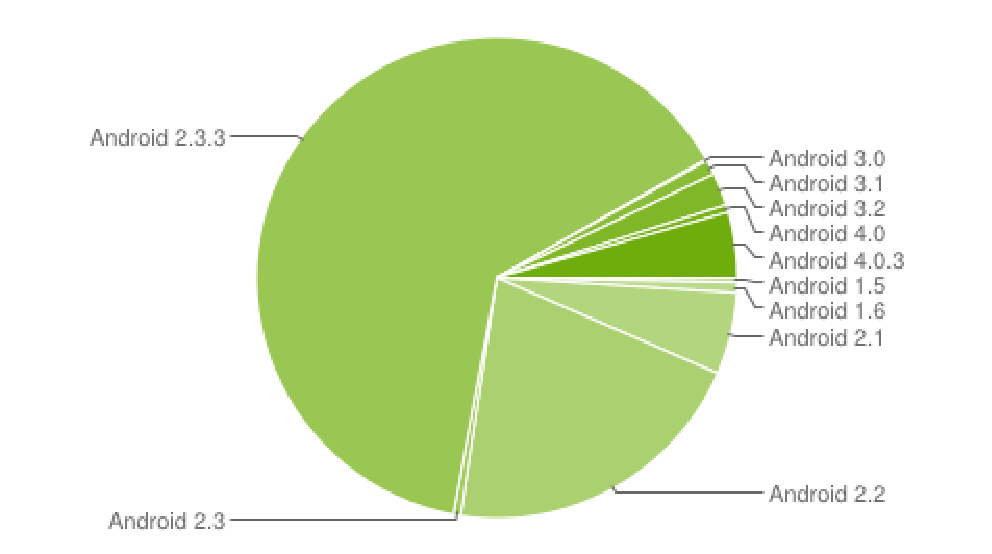
\includegraphics[scale=0.3]{/home/coach/Dropbox/RTOS/Android_chart}

\label{Android distribution diffusion}

We can notice that now the common kernel distributions still use Linux
2.6.x kernel.

Figure \ref{Android structure} shows Android System Architecture
schema \cite{WIKI}.

\includegraphics[scale=0.3]{/home/coach/Dropbox/RTOS/System-architecture}

\label{Android structure}

Android \cite{OVERVIEW} provides some modification to main Linux
kernel, such as an improved power management, ASHMEM virtual memory,
some specific-component drivers, and a low memory killer. The latter's
mission is to free memory when the system run Out of Memory (OOM).

%-----------------------------------------------------------------------------


% TODO: 
 - ampliare l'introduzione
 - rivedere parte su CMA: guardarsi gli altri articoli, condensare le notizie importanti
 - finire ION con gli sviluppi futuri: integrazione CMA con ION.
 - TUTTA la parte su OOM killer
 - 


\subsection{Low level management and integration with HW resources}

In this part, we discuss about how the memory has managed in Android
devices. For most of the releases in Android, it was used PMEM and
ASHMEM. These kind of libraries was too simple, and was patched with
some SoC patches, such as NVMAP for nVidia Tegra devices and CMEM
for TI OMAP ones. The most important patch was CMA (Contiguous Memory
Access), expecially with DMABUF patch. With the release of Android
4.0 (Ice Cream Sandwich) a brand new driver has released, ION. We
discuss about differences between ION and CMA approach, and, in the
state-of-art, we discuss of a future integration between them.

%-----------------------------------------------------------------------------



\subsection{PMEM and ASHMEM}

PMEM (Process MEMory)\cite{AKF} is the first memory driver implemented
on Android devices (since G1). It is used to manage shared memory
regions sufficiently large (from 1 to 16MB).

This regions must be physically contiguous between user space and
kernel drivers (such as GPU, or DSP). It was written specifically
to be used in a very limited hardware platform, and it could be disabled
on x86 architectures.

ASHMEM\cite{ASHMEM} (Android SHared MEMory) is a shared memory allocator
subsystem, similar to POSIX, but with a different behavior. It also
gives to the developer an easier and file-based API. It used named
memory, releasable by the kernel. Apparently, ASHMEM supports low
memory devices better than PMEM, because it could free shared memory
units when it is needed. 

\begin{tabular}{|>{\centering}p{0.33\columnwidth}||>{\centering}p{0.4\columnwidth}|}
\hline 
PMEM & ASHMEM\tabularnewline
\hline 
\hline 
Uses physically contiguous addresses & Uses virtual memory\tabularnewline
\hline 
\hline 
The first process who instantiate a memory heap must keep that till
the last one of the users won't free the file descriptor. Thus to
preserve contiguity & Memory is handled by instances (object oriented like). It is managed
by a reference counter\tabularnewline
\hline 
\end{tabular}


\subsection{CMA and DMABUF}

CMA (Contiguous Memory Allocator)\cite{CMAdoc} is a well known framework,
which allows setting up a machine-specific configuration for physically-contiguous
memory management. Memory for devices is then allocated according
to that configuration. Differently from similar framework, it let
regions of system-reserved memory to be reused in a transparent way,
letting memory not to be wasted. When an alloc is instantiated, this
framework migrates all the system page. Thus to build a big chunk
of physically contiguous memory.

Why do an OS have to use chunks of memory?\cite{CMA,RCMA} Because
virtual memory tends to fragment pages. An intensive use of memory
let the system not able to find contiguous memory in a very short
time after boot. Recently, the requirement of huge pages in applications
raises, especially for transparent huge pages. Another question is
devices (such as cameras) that needs DMA over areas physically contiguous.
CMA reserve an huge area of memory at boot time, only for huge request
of memory. For every region, block of pages can be flaggable as three
type. 
\begin{itemize}
\item movable : typically, cache pages or anonymous pages, accessed by page
table or page cache radix tree 
\item kernel recallable : they can be given back to the kernel by request. 
\item immovable : these are typically pointer referred pages (such as pages
invoked by a kmalloc()) 
\end{itemize}
The memory manager subsystem try to keep movable pages as near as
possible. Grouping these pages, kernel try to ensure more and more
contiguous free space available for further request. CMA extends this
mechanism. It adds a new type of migration (CMA). Pages flagged as
cma behave like the movable ones, with some differences: 
\begin{itemize}
\item they are ``sticky'' 
\item Their migration type can't be modified by the kernel 
\item In CMA Area, the kernel cannot instantiate pages not movable.
\end{itemize}
In other words, memory flagged as CMA keep available for the rest
of the system with the only restriction to be movable. 

When a driver ask for a huge contiguous allocation of memory, CMA
allocator can try to free in his own area some contiguous pages to
create a buffer large as needed. When the buffer is no longer requested,
memory can be used for other needs. CMA can just take only the needed
amount of memory without worrying about strictly request of alignment.

DMA buffers has different request despise of huge pages.

\begin{tabular}{|>{\centering}p{0.33\columnwidth}|>{\centering}m{0.33\columnwidth}|}
\hline 
DMABUF & Transparent Huge Pages\tabularnewline
\hline 
\hline 
Normally larger than Transparent Huge Pages. 10 Mb.

It could be needed specific memory area, if underlying hardware is
sufficiently ``strange'' & Almost 2Mb large\tabularnewline
\hline 
DMA requires less alignment than THP & 2MB of THP needs 2Mb of Alignment\tabularnewline
\hline 
\end{tabular}

CMA patches provides a set of function that can prepare regions of
memory and the creation of contest area of a well known size using
function cm\_alloc and cm\_free to keep and release buffers. CMA must
not be invoked by the driver, but from DMA support functions. When
a driver call a function like dma\_alloc\_coherent(), CMA should be
invoked automatically to satisfying the request. This should work
in normal condition.

One of the issue about CMA is how to initially alloc this area of
memory. Current scheme needs that some of special calls should be
done by the board file system, with a very arm-like approach. The
idea is to do that without board files. The ending result is that
it should be at least one iteration of that patch set before it will
be executed by the mainline. 


\subsection{ION}

In december 2011, PMEM is marked as deprecated, and then replaced
by ION memory allocator\cite{ION}. ION is a memory manager that Google
has developed from the 4.0 release of Android (Ice Cream Sandwich),
mainly to resolve the interface issue between different memory management
between different Android device. In fact, some SoC developer implemented
different memory manager. We can cite some of them:
\begin{itemize}
\item NVMAP, implemented on nVidia Tegra 
\item CMEM\cite{CMEM}, implemented on TI OMAP 
\item HWMEM\cite{HWMEM}, implemented on ST-Ericsonn devices 
\end{itemize}
All this vendor will pass to ION soon

Besides ION being a memory pool manager, it also enables his clients
to share buffers (so, it works like DMABUF, the DMA buffer sharing
framework). Like PMEM, ION manages one or more pools of memory, some
of them instantiated at boot time or from hardware blocks with specific
memory needs. Some devices like that are GPU, display controllers
and cameras. ION let his pools to be available as heap ION. Every
kind of android device can have different ION heaps, depending on
device memory. Phisical address and heap dimension can be returned
to the programmer only if the buffer is physically contiguous. Buffer
can be prepared or deallocated to be used with DMA, or with virtual
kernel addressing. Using a file descriptor, it can be also mapped
in the user-space. There are three kind of allocable ION heap. Other
ones can be defined by SoC producers (like ION\_HEAP\_TYPE\_SYSTEM\_IOMMU
for hardware blocks equipped with IOMMU driver). 
\begin{itemize}
\item ION\_HEAP\_TYPE\_SYSTEM
\item ION\_HEAP\_TYPE\_SYSTEM\_CONTIG
\item ION\_HEAP\_TYPE\_CARVEOUT : in this case, carveout memory is physically
contiguous and set as boot. 
\end{itemize}
Typically, in the user-space case, libraries uses ION to alloc large
continuous buffers. For instance, camera library can alloc a capture
buffer to be used from the camera device. Once the buffer is fulfilled
with video data, the library gives the buffer to kernel to be processed
by jpeg encoder block. A c/c++ program must have access to '/dev/ion'
before it can alloc memory thanks to ION. He can alloc data using
file descriptors (fd). It can be maximum one client for user process.

Clients interacts from user-space with ION using ioctl() system interface.
Android processes can share memory using their fd. To obtain shared
buffer, the second user process must obtain a client handle through
a system call open('/dev/ion', O\_RDONLY). ION manage user space client
through process PID (in particular, the 'group leader ' one). Fd will
be instantiated pointing at the same client structure in the kernel.
To free a buffer, the second client must invalidate the mmap() effect,
with an explicit call at munmap(), and the first client must close
the fd, calling ION\_IOC\_FREE. This function decrements the reference
counter of the handle. When it reaches zero, the ion\_handle is destroyed,
and the data structure that manages ION is updated. While managing
client calls, ION validates input from fd, from client and from handler
arguments. This validation mechanism reduce the probability of undesired
access and memory leaks. Ion\_buffers is somewhere similar to DMABUF.
Both uses anonymous fd, reference counted, as shareable objects.

\begin{tabular}[t]{|>{\centering}p{0.2\columnwidth}|>{\raggedright}p{0.4\columnwidth}|>{\raggedright}p{0.3\columnwidth}|}
\hline 
 & ION buffers & DMABUF\tabularnewline
\hline 
\hline 
Application level MMU & Alloc and free memory from memory pools in a shareable and trackable
way & It focus on import, export and syncronization in a consisten way with
buffer sharing solution for non arm architectures\tabularnewline
\hline 
Role of Memory manager  & ION replace PMEM as memory pools manager. ION heap lists can be extended
by the device.  & DMABUF is a buffer sharing framework , designed to be integrated with
memory allocator in contiguous DMA mapping framewors, such as CMA.
DMABUF exporters can implement custom allocator.\tabularnewline
\hline 
User Space access control  & ION offers /dev/ion interface to user space program, letting them
to alloc and share buffers. Every user process with ION access can
suspend the system overlapping ION heap. Android chech user and groupID
blocking non authorized access to ION heap & DMABUF offers only kernel API.

Access control is a function of the permissions on device that uses
DMABUF feature\tabularnewline
\hline 
Global Client and Buffer Database.  & ION has a driver associated to /dev/ion. The device structure has
a database that keeps ION buffers allocated, handlers and fd, grouped
by user client and kernel client. ION validates all the client calls
to be valid for database rules. For instance, an handle can't have
two buffers associated. & The debub structure of DMA implements a global hashtable, dma\_entry\_hash,
tracking DMA buffers, but only when kernel is build with CONFIG\_DMA\_API\_

DEBUG option.\tabularnewline
\hline 
Cross- architecture usage & ION usage now is limited on architectures that runs kernel Android & DMABUF usage is cross architecture. DMA mapping redesign let his implementation
in 9 architectures beside the ARM one. \tabularnewline
\hline 
\end{tabular}

\begin{tabular}[t]{|>{\centering}p{0.18\columnwidth}|>{\centering}p{0.35\columnwidth}|>{\centering}p{0.33\columnwidth}|}
\hline 
 & ION\_buffer & DMABUF\tabularnewline
\hline 
\hline 
Buffer Syncronization & \multicolumn{1}{>{\centering}p{0.35\columnwidth}||}{Ion consider the syncronization problem as an orthogonal problem} & DMABUF gives a pair of API for synchronization. Buffer user invokes
dma\_buf\_map\_

attachment() everywhere he desires to use buffer for DMA. Once he
finished using that, signals \textquotedbl{}endOfDMA\textquotedbl{}
to exporter using dma\_buf\_unmap\_

attachment()\tabularnewline
\hline 
\hline 
Buffer delayed allocation & ION allocs physical memory before the buffer is shared & DMABUF can delay allocation till the first call of dma\_buf\_map\_

attachment(). DMA buffer exporter has the opportunity of scans every
client attachment, collecting all the constraints and choose the most
efficient storage\tabularnewline
\hline 
Integration with Video4

Linux2 API  & Processes that uses these API tends to use PMEM. So, the migration
from PMEM to ION has a relatively small impact. & DMABUF integration with Video4Linux is hard and asked for lots of
modifies in DMABUF. But in a long time that will be a smart choice,
because DMABUF sharing mechanism is fitted for DMA, so it is well
written for CMA and IOMMU. Both of them reduces carveout memory needs
to build an Android smartphone.\tabularnewline
\hline 
\end{tabular}


\section{OOM Killer}


\subsection{Introduction}

Mobile devices become more and more rich of memory over time, due
to Moore's Law. However, there's always a limit over wich memory isn't
available, and a well form kernel needs some politics to free bunch
of memory when needed. Android provides an OOM killer, who kills processes
using heuristics, developed over time.\cite{OOM_TAMING}

%%copincollato dall'articolo!

Major distribution kernels set the default value of /proc/sys/vm/overcommit\_memory
to zero, which means that processes can request more memory than is
currently free in the system. This is done based on the heuristics
that allocated memory is not used immediately, and that processes,
over their lifetime, also do not use all of the memory they allocate.
Without overcommit, a system will not fully utilize its memory, thus
wasting some of it. Overcommiting memory allows the system to use
the memory in a more efficient way, but at the risk of OOM situations.
Programs that asks lots of memory can consume all the system's memory,
stopping the whole system. This can lead to a situation, when memory
is so low, that even a single page cannot be allocated to a user process,
to allow the administrator to kill an appropriate task, or to the
kernel to carry out important operations such as freeing memory. In
such a situation, the OOM-killer kicks in and identifies the process
to be killed for the benefit of the rest of the system.


\subsection{OOM euristics}

To facilitate OOM system control, the /proc/<pid>/oom\_adj knob was
introduced to save important processes in the system from being killed,
and define an order of processes to be killed. The possible values
of oom\_adj range from -17 to +15. The higher the score, more likely
the associated process is to be killed by OOM-killer. If oom\_adj
is set to -17, the process is not considered for OOM-killing.

Who's Bad? The process to be killed in an out-of-memory situation
is selected based on its badness score. The badness score is reflected
in /proc/<pid>/oom\_score. 

This euristic value is determined on the basis of four characteristics:
\begin{itemize}
\item that the system loses the minimum amount of work done, 
\item recovers a large amount of memory, 
\item doesn't kill any innocent process eating tons of memory, 
\item kills the minimum number of processes (if possible limited to one)
\end{itemize}
The badness score is computed using 
\begin{itemize}
\item the original memory size of the process, 
\item its CPU time (utime + stime), 
\item the run time (uptime - start time) 
\item its oom\_adj value. 
\end{itemize}
The more memory the process uses, the higher the score. The longer
a process is alive in the system, the smaller the score.

Any process unlucky enough to be in the swapoff() system call (which
removes a swap file from the system) will be selected to be killed
first. For the rest, the initial memory size becomes the original
badness score of the process. Half of each child's memory size is
added to the parent's score if they do not share the same memory.
Thus forking servers are the prime candidates to be killed. Having
only one \textquotedbl{}hungry\textquotedbl{} child will make the
parent less preferable than the child. Finally, the following heuristics
are applied to save important processes:
\begin{itemize}
\item if the task has nice value above zero, its score doubles 
\item superuser or direct hardware access tasks (CAP\_SYS\_ADMIN, CAP\_SYS\_RESOURCE
or CAP\_SYS\_RAWIO) have their score divided by 4. This is cumulative,
i.e., a super-user task with hardware access would have its score
divided by 16. 
\item if OOM condition happened in one cpuset and checked task does not
belong to that set, its score is divided by 8. 
\item the resulting score is multiplied by two to the power of oom\_adj
(i.e. points <\textcompwordmark{}<= oom\_adj when it is positive and
points >\textcompwordmark{}>= -(oom\_adj) otherwise). 
\item The task with the highest badness score is then selected and its children
are killed. The process itself will be killed in an OOM situation
when it does not have children.
\end{itemize}
%%che ne dici di un bel grafico riassuntivo qui?


\subsection{User space OOM killer control }

There's a problem in using purely heuristics: value of /proc/<pid>/oom\_score
is dynamic and very difficult to guess. Also, it could not be as flexible
as an administrator needs. It is difficult to determine which process
will be killed in case of an OOM condition. The administrator must
adjust the score for every process created, and for every process
which exits. This could be quite a task in a system with quickly-spawning
processes. In an attempt to make OOM-killer policy implementation
easier, a name-based solution was proposed.

With his patch, the process to die first is the one running the program
whose name is found in /proc/sys/vm/oom\_victim. A name based solution
has its limitations:
\begin{itemize}
\item task name is not a reliable indicator of true name and is truncated
in the process name fields. 
\item Moreover, symlinks to executing binaries, but with different names
will not work with this approach 
\item This approach can specify only one name at a time, ruling out the
possibility of a hierarchy 
\item There could be multiple processes of the same name but from different
binaries. 
\end{itemize}
The behavior boils down to the default current implementation if there
is no process by the name defined by /proc/sys/vm/oom\_victim. This
increases the number of scans required to find the victim process.\bibliographystyle{savetrees}
\nocite{*}
\bibliography{Report}


\end{multicols} 
\end{document}
